\chapter{Background and Research Domain}


One of the most widely-used features of Twitter is its inbuilt function for easily facilitating the spread of information through its social structure. This phenomenon is the basis for much of the research in this thesis and, when combined with the characteristics of Twitter's user graph, has many interesting attributes and behaviours associated with it.


\section{Domain Introduction and Literature Survey}
This section provides an understanding of retweeting in Twitter and its effects on the users and the followships between them, which represent the underlying social graph of Twitter, and includes a survey of some of the most relevant works of the area.

\subsection{Information Propagation through Retweeting}
The function of propagation in Twitter is known as \textit{retweeting}, and is carried out by the Twitter users themselves. When a user views a Tweet that they believe to be particularly interesting, and believe it to also be interesting to his/her followers, then he/she can elect to retweet it, and thus pass it further through the social graph to that user's followers also. A Tweet that has been retweeted is known as a \textit{retweet}, and it is clear that a Tweet which is retweeted will be made available to significantly more users than a Tweet that isn't retweeted \cite{webberley11} \cite{kwak10}. Since Twitter's social graph is decentralised and retweeting occurs between individual groups of users, its properties are similar to information dissemination in other types of decentralised graphs, such as content-forwarding in opportunistic networking \cite{allen10}.

A retweet can be carried out in one of two ways: either through the use of Twitter's native retweet `button', or manually. The button is displayed along with each Tweet (see Figure \ref{fig:retweet_button}) in a timeline which, when clicked, immediately creates a new retweet containing the verbatim content of the original Tweet and automatically sends it on to the retweeting user's followers. The user who created the original Tweet is credited as the author on the recipients' timelines, with an indication of who carried out the retweet itself. Thus, users who follow the retweeter will see a Tweet appear in their home timeline from someone that they may not directly follow. Figure \ref{fig:northern_lights_tweet} illustrates an example; the user receiving the depicted Tweet does not follow the original author, \texttt{@aldakaida}, but \textit{does} follow \texttt{@DTW\_Holidays}, who was responsible for carrying out the retweet. 

\begin{figure}[h]
\centering
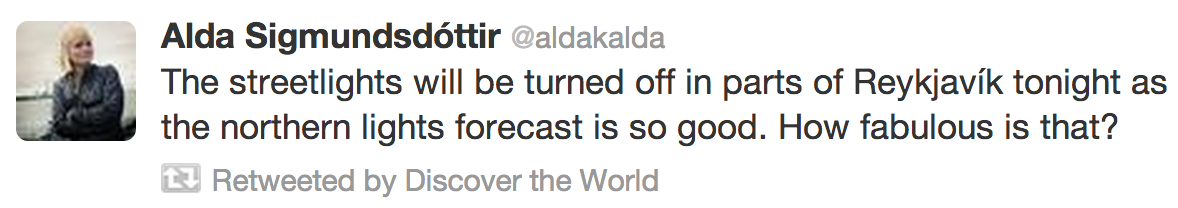
\includegraphics[scale=0.3]{2.Background/Media/northern_lights_tweet.png} 
\caption{A retweeted Tweet.}
\label{fig:northern_lights_tweet}
\end{figure}

The manual approach involves physically copying the content of the Tweet to be retweeted and pasting it into a new Tweet, usually with the text `\texttt{RT @<username>:}' pre-pended, where \texttt{RT} stands for \textbf{r}e\textbf{t}weet and \texttt{<username>} is the username of the author of the original Tweet. This method allows for annotating the original content of the Tweet (for example, to provide an opinion on the Tweet contents), producing a \textit{modified} Tweet, which can sometimes be pre-pended with \texttt{MT} rather than \texttt{RT}.

Historically, this manual approach was informally community-driven by the users of Twitter and was the only method available for carrying out retweets. However, in 2009, Twitter realised the popularity of this user convention and introduced the retweet button\footnote{https://blog.twitter.com/2009/project-retweet-phase-one} in order to assist in this trend, and through which Tweets could be retweeted much more quickly and accessibly. The button is implemented on Twitter's website and mobile device applications, yet even today the original and manual retweet approach remains popular amongst many of Twitter's users and communities.

\begin{figure}[h]
\centering
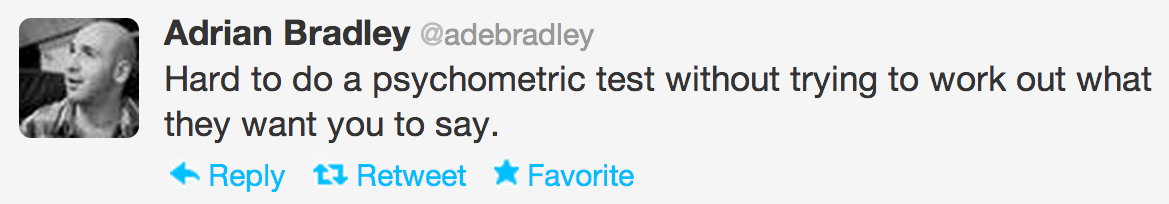
\includegraphics[scale=0.3]{2.Background/Media/retweet_button.png} 
\caption{The retweet `button' in context.}
\label{fig:retweet_button}
\end{figure}

Each Tweet has a retweet count associated with it, which is the raw representation of the number of times that the Tweet has been retweeted using the retweet button method. Since the manual retweet technique remains more community-driven, there is no official way to include these as part of the retweet count of the original Tweet. However, since the manual method is typically only used with the aim to annotate or modify the Tweet in some way, the resultant `retweet'  is no longer a real representation of the content of the original Tweet, and so should not be counted as such.

It should be noted that Twitter users may choose to make their account `protected'. A person who has a protected account will still have a publicly-visible profile (displaying a name, username, bio, and so on), but their Tweets and other information (such as the followers and friends lists) are hidden from users that aren't followers of the person. Potential followers of a protected account must \textit{request} a followship, which can then be accepted or rejected by the protected account holder. Since Tweets from a protected account are only visible to approved followers, the retweet button is unavailable for them to disseminate the Tweet any further than the author's immediate local follower network. However, since the manual retweet method does not rely on the button and isn't governed by Twitter, a protected account's Tweets can still be retweeted in this way.

As Facebook supports the endorsement of information found on its site by inviting users to `like' a piece of content, retweeting is effectively a \textit{vote} or endorsement for a Tweet on Twitter. In both cases, the number of likes and number of retweets is available to the platforms' respective users (Figure \ref{fig:tweet_comparison}), and so this provides some insight into the \textit{popularity} of the information. Whilst Facebook `likes' are immediately visible to users in feeds, the retweet count becomes visible once a user clicks a Tweet to expand its metadata.

Some Twitter users declare that their `retweets are not endorsements' in their profile's bio. This particular behaviour is largely associated with journalists who use retweets to highlight potentially controversial Tweets and to ignite discussion over certain topics. This declaration is unwelcomed by some users, who then argue the point by asking what retweets \textit{are} meant to imply\footnote{http://www.poynter.org/latest-news/media-lab/social-media/152448/the-problem-with-retweets-how-journalists-can-solve-it/} and that a user's bio is not immediately available for recipients to view in Tweet streams. Generally, this is not very widespread, and even Tweets retweeted with the aim of not being an endorsement imply some level of \textit{popularity} of the Tweet. 


\subsection{Retweets and the Social Graph}
The social graph of Twitter can be represented, like other online social networks, by edges between users, partially emulating real-life social interactions between humans. The growth of social media has encouraged more dense communication between users all over the world, who would not previously be able to be in direct contact with one another in this way.

Stanley Milgram's ``six degrees of separation'' \cite{milgram67} experiments are highly relevant to and useful for OSN research today. The results of the experiments demonstrated that people are usually no more than six hops away from each other on the world's social graph, yet this value was found to be an overestimate when it comes to the analysis of the structure of OSNs by \cite{backstrom11}, who found that the average `distance' observed in Facebook's entire 721 million-node graph in 2011 was only around 4.7 hops. This implies that denser links between users and larger communities that apparently manifest themselves in OSNs create a smaller `world' than that experienced in reality.

In each of Milgram's experiments participants passed a message to one another, at each stage only passing to other people that they actually \textit{know}, in the hope of the it reaching a single intended recipient. This meant that people could use acquaintances in other geographic locations to transfer the message from community to community. Twitter supports a similar propagation mechanism in the fact that retweets can themselves be retweeted; this is a focus of some of the earlier research in this thesis.

This behaviour provides further penetrative `depth' of the information through the social network away from the source user in addition to the spread `width' made by the initial retweets. Although retweeting is not carried out with the aim of information reaching any particular final user (or set of users), as with Milgram's experiment, this phenomenon allows retweets to `travel' between `online communities' of users.

As with real-life social networks, communities of users in OSNs are also a common feature \cite{ugander11}. Social communities are identified by clusters of people sharing dense links with each other, and can vary in size, location, and geographic spread. They often grow over time and are formed between people living near to each other or between groups of users with shared interests.

In Twitter, these communities are typically small to begin with and are based on a topic of interest or around a more influential user. As Tweets are produced from within the community, further links are made to interconnect the community's users, producing a growing `swarm' of interest around the initial topic or user \cite{java07}. As further users begin associating themselves with this community, its audience becomes widespread and the community grows. This concept is discussed in greater length by \cite{java07}, who also experiment further with communities and describe them as compact groups of users connected by dense follower links.

\begin{figure}[h]
\centering
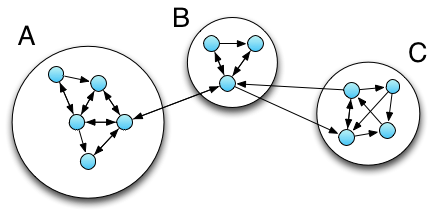
\includegraphics[scale=0.7]{2.Background/Media/communities.png} 
\caption{A hypothetical group of user communities.}
\label{fig:communities}
\end{figure}

In more dense communities, Tweets can be made available to many users immediately after they are published, since many of the links between users are shared. This means that any retweets that occur within communities are likely to have a lot of \textit{redundancy}, in that many of the retweets will be sent to users who have already seen the original Tweet. Twitter prevents this information duplication by not displaying the retweets of Tweets that have already appeared on a user's timeline. However, this does increase the chance of the Tweet being propagated to users external to the community.

Retweets amongst users within a community are likely to be common, due to the shared-interest nature of communities, and some users can provide `bridges' by being active in more than one group. In these cases, Tweets can be passed between the communities through retweets by the bridging user. For example, Figure \ref{fig:communities} illustrates three hypothetical communities `bridged' by one user in community B. If this user was to retweet a Tweet from communities A or C, then it is clear how the Tweet could be propagated from one group of users to another. If there are many users sharing communities then there are many more avenues available for dissemination through the graph, causing a high level of information throughput. If there are fewer bridges, then there is more of a bottleneck between the communities, hindering the information spread.

\cite{java07} also finds that communities can be formed from different types of people, such as those who Tweet frequently and have many followers, and those who contribute very little and have few followers. Those with many followers and many friends receive lots of information and have the potential to spread information further than those with fewer inward and outward edges. Studies in the behaviour of different types of users in Twitter is more thorough in \cite{krishnamurthy08}, which defines `broadcasters' (users with many followers and few friends) and `miscreants' (users with few followers but many friends) and their roles in information propagation. The authors desribe broadcasters as users who post many Tweets, which are then received by large numbers of users, and miscreants as those who receive lots of information but are unable to achieve a large Tweet audience. It is therefore assumed that broadcasters are likely to be retweeted more than many other types of user.

Users that retweet the interesting information from a source user to others, who do not follow the source user and so would not naturally receive the information, are effectively acting as information \textit{filters}. By not following the source user, a person might still receive the interesting information through these filters, but will not receive any of the `noise'. Thus retweeting means that friends of a user become useful filters of information for users further `downstream'  and retweeted information can be said to have a higher \textit{credibility} than Tweets that aren't retweeted \cite{castillo11}.


\subsection{User Influence}
Just as there are different types of user \textit{behaviours} on Twitter, there are also users of different \textit{influence} levels \cite{quercia11}. Much research has gone into user influence, including on how this might be detected \cite{yu11}, and influential users are generally found to be those who have a greater impact on Twitter's social network \cite{bakshy11} and who usually have significantly more followers than an average user. Influential users tend to have a high persuasion over other users, relating \textit{influtentials} in Twitter to those who are also influential in the real world as part of traditional communication theory \cite{cha10}, and therefore many Twitter influentials are the accounts belonging to real-world celebrities.

As with real-world celebrities, Twitter influentials are those with many `influenced' followers, or fans, which are the users who have the strongest agreeable opinions of the influential. As a result, an influential user has a greater number of followers who are interested in the information produced by the user, and is therefore more likely to receive more retweets than less influential users.

Although influence level is partly derived from the follower count of the user, it should be noted that a user with high in-degree on the social graph\footnote{In-degree: many followers} does not necessarily imply a high level of influence. An `active' audience of users who reply, retweet, and interact are more indicative of an influential user \cite{bigonha10}. This is especially true since a user can gain more followers through campaigns such as `\#teamfollowback'\footnote{Users associate themselves with \#teamfollowback to imply they will return all followships.} or by following `out of politeness', in which a user will follow another user back as an act of politeness, but these users tend to have \textit{both} high in- and out-degree and invoke less interactivity amongst their followers, which are not necessarily characteristics of an influential user \cite{cha10}.

Klout\footnote{http://klout.com} is a web service that attempts to review a user's social media influence by assigning users a Klout Score. Their website declares that this score, which ranges from 0 to a maximum of 100 and whose generation algorithm is kept private and unpublished \cite{edwards13}, is determined from a variety of over 400 `signals' taken from eight different social media platforms. These signals are derived from various attributes including the volume of information shared, the reaction to the shared information, and the relative scores of the users who interact with the information. They \textit{also} take interactivity between users as one of the primary indicators \cite{anger11}. Additionally, the service indicates the topics a user is influential about, with the general idea being for organisations to check up on which users are influential for marketing purposes, but also to highlight the users that should be replied-to at a higher priority.


\subsection{Twitter as an Information Retrieval System}
At a high level, Twitter can be considered a variety of information-retrieval system, which people can utilise to produce and consume information when required. In traditional information-retrieval systems, such as search engines and library systems, keywords and search terms are common ways for describing the type of information the user would like to receive. The system would then search a database or archive for what it believes is relevant information, \textit{based} on these `retrieval parameters', and return results to the user ordered usually by the estimated relevance of the articles \cite{arvola10}.

Information quality is also reliant on the expected reading effort of the returned documents. The character precision-recall metric was introduced by \cite{arvola10} by way of demonstrating the tolerance-to-irrelevance ratio. The general mechanism for this ratio is to do with users reading a document passage; the point at which this ratio is reached is when the user stops reading the particular passage and moves to the next whole document, since they assume the rest of the document is also irrelevant to them. Therefore, the more effective the information retrieval system is in displaying high-quality information, the lower the chance that this ratio is reached by the user. This is comparable to the event in which a Twitter user viewing Tweets from someone they are following gets to the point where he or she reaches this ratio (i.e. is beginning to get bored or find the Tweets irrelevant) and decides to unfollow the friend. Similarly, the more effective the user is when selecting people to follow in the hope of receiving interesting information, the less likely it is that the user will remove these friends.

Whilst Twitter does not support the use of keyword searching for its primary information delivery method, it does lend its users some control over the type of information they wish to receive. As mentioned previously, users receive all of the Tweets from everyone that they follow onto their home timelines. Thus, by selecting users to follow, a person is effectively describing and implicitly indicating the type of information he/she would like to receive, and by editing their friends list (either by adding new followers or pruning existing ones) he/she can alter this indication. In addition, Twitter moves towards an information-\textit{recommendation} system, in that the friends of a user can endorse and imply a Tweet's quality by retweeing it.

Despite this control, it is still unlikely that users will achieve a perfect Twitter experience due to the presence of \textit{noise} \cite{alonso10}. As discussed in the Introduction, this problem stems from that although a person follows users they consider to be interesting, it is often the case that not \textit{all} information produced by interesting users will be interesting itself. For example, a user may follow a news source in order to receive breaking news but is not interested in viewing the information about politics or celebrity updates that the news source also Tweets about.


\subsection{Information Quality, Popularity and `Interestingness'}
The concept of interestingness in online social networks is based around information that conveys some \textit{affective stimulation} to the viewer, as is described in further detail in Section \ref{section:affective_stimulation}. Generally, interestingness is subjective as it takes into account features such as a person's interest in the topic of the information and how \textit{relevant} the information is to the viewer. However, in this thesis, interestingness is used to describe information that is not noise and contains some amount interesting information. As such, this research is aimed towards the identification of information from the noise surrounding it that might be of relevance to viewers.

Information-retrieval systems typically use some measure of information \textit{quality} when determining which documents to return to a user and also when deciding on the \textit{order} the documents should be displayed in. This `quality' is subjective in that different systems use a variety of different algorithms for deducing quality, usually based on the level of \textit{interest} in each of the available documents (such as Google's Page Rank algorithm and Amazon's recommendation algorithms), but also in that the level of quality itself depends on the user itself requesting the information. 

In the case of Google's Page-Rank, the algorithm uses multiple cues to determine who the user is, their interests, past searching habits, links clicked, and so on, to return \textit{relevant} information, which is incidentally one of the causes of the aforementioned Google search bubble. Amazon's recommendation algorithms analyse a user's past item views and purchases and cross-matches these against trends based from users who also looked or bought similar items. Amazon is then able to accurately determine the type of items a customer are interested in purchasing, and can send emails to that customer with personalised recommendations. In these cases, information quality is essentially a function of information interestingness and information relevance.

Twitter uses no such metrics to deliver information to its users, relying on the users themselves to implicitly `choose' the information they want to receive. Additionally, information is always displayed in chronologically-ordered timelines, with new Tweets being continuously inserted at the top as they occur. Twitter does not try to indicate interesting Tweets on the timeline which means that the interesting information is shown at equal value alongside the `noisy' Tweets, causing the difficulties in identifying the interesting information as has been mentioned previously. Indeed, the recent TechCrunch article from October 2013, ``Twitter Quitters And The Unfiltered Feed Problem''\footnote{http://techcrunch.com/2013/10/05/sorry-my-feed-is-full} talks at more length about this particular phenomenon, and helps highlight the problem area of this work more clearly from a layperson's perspective.

The retweet count of a given Tweet is a useful metric in inferring a its \textit{popularity}. If a Tweet is retweeted 10 times, then ten people have taken the time to read that Tweet, decide it is worth sharing, and then actually retweet it \cite{uysal11}. This user (and the other nine retweeters) may have found the Tweet interesting, yet it should be noted that although the count can be used as a measure of popularity, as a function of the influence of the Tweet's author, the retweet count alone cannot be used as a measure of how interesting the Tweet actually is \cite{naveed11}. For example, it is inappropriate to say that the first Tweet in Figure \ref{fig:tweet_comparison} is so significantly more \textit{interesting} than the second, although it is clearly more popular since Justin Bieber is an extremely influential Twitter user.

\begin{figure}[h]
\centering
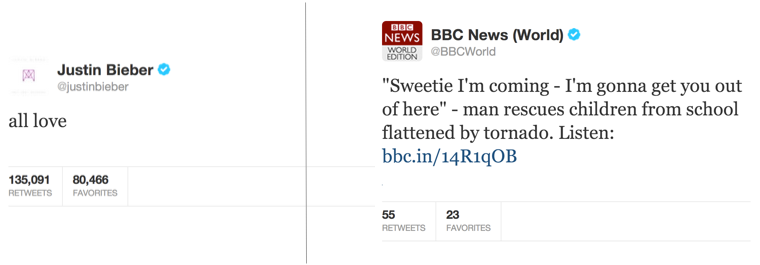
\includegraphics[scale=0.55]{2.Background/Media/compared_tweets.png} 
\caption{Example of Tweets with significantly different retweet counts.}
\label{fig:tweet_comparison}
\end{figure}

Whilst the work in this thesis does not primarily aim to build an accurate retweet-predictor, this does become more important in some of the work in later chapters, since it forms part of the basis of the methods of interestingness inference as a function of many retweet \textit{decisions}. \cite{uysal11} also identifies the problem of `noisy' Twitter timelines and discusses methods for predicting \textit{popular} Tweets using a J48 decision tree classifier, based on the likelihood of the Tweet being retweeted by a particular user. Although the authors address information relevance from a user-centric point of view, the validation of whether a prediction of a retweet occurring for a given Tweet is actually indicative of the \textit{interestingness} of said Tweet do not perform particularly well.

A retweet-prediction model based on a factor graph model is introduced by \cite{yang10} to determine how retweetable a Tweet is on a global scale. A precision of just under 29\% is achieved in predicting if a Tweet will be retweeted, but no mention is made of how this relates to how \textit{interesting} the information is. Another study into retweet prediction was carried out by \cite{zaman10}, in which a trained probabilistic collaborative filter model (named `Matchbox') was used to determine the useful features in making the predictions. As with the previous study, the research focuses on a retweet \textit{probability}, which is a binary decision made by one particular user. The methodology is not aimed at the inference of interestingness, and simply determines that the most relevant features for accurate decision predictions are the author of the original Tweet and the retweeter.

Inversely, \cite{suh10} and \cite{hong11} predict the \textit{type} of messages that are likely to be retweeted further, the latter using a logistic regression to both predict an individual retweet decision and a retweet \textit{volume}. The methods do not apply these notions to how interesting the information actually is to a particular user, achieve low recall and the multi-classifications seems only to perform well on very unpopular or very popular Tweets. It is made clear, however, that the retweet volume of a Tweet is useful in denoting Tweet \textit{popularity}.

\cite{petrovic11} uses a passive-aggressive machine-learning algorithm to make binary predictions on retweet decisions and cited that social features - for example, number of followers of the author, frequency of Tweeting, etc. - were the largest factors in the performance, and \cite{naveed11} uses a logistic regression, partly using a dataset published as part of another paper by the same authors as \cite{petrovic11}, to predict retweet decisions in order to address information interestingness. However, little effort is made to define interestingness or, indeed, validate that the inferences towards this are accurate and correct. A logistic regression is again used by \cite{zhu11} for predicting binary retweet behaviours with the focus on information propagation in disaster scenarios, and \cite{peng11} showed that conditional random fields can perform better than logistic regressions when modelling retweet behaviour in the same way.

Since the above papers only effectively consider a prediction of retweet outcome, which is a binary decision, it is hard to relate this more to the notion of global interestingness, aside from stating that a retweet implies the retweeter's relative interest in the Tweet. However, a retweet count, as mentioned above, is inappropriate as an indicator of \textit{magnitude} of interest, and so the research into predicting individual retweet decisions cannot be used as a basis for this. Additionally, not much emphasis is placed on how well the techniques work on a more `on demand' basis; many of the methodologies discussed require several features that may take a long time to collect and compute, making them unsuitable for use as part of quick and useful interestingness evaluations.

The idea of Tweet scoring and retweet \textit{count} predictions is introduced by \cite{gransee12}, who used their methodologies to produce a system\footnote{https://sites.google.com/site/learningtweetvalue/home} enabling users to compile Tweets in ways that are predicted to achieve the most retweets. The predictions are based on averaging the score, derived through a linear regression, of different components of a user's Tweets (such as the inclusion of a particular hashtag), so that when a Tweet by the same author is next constructed, the various components of the new Tweet can be compared against the scores of the counterparts seen in previous Tweets. The value produced through this method is then used to generate an expected retweet count as part of a comparison to the user's average (`baseline') achieved retweet count at this point in time, and was shown to perform well on influential Twitter users.

However, the methods described do not take into account fluctuations in the social graph, particularly in the case of less-influential Twitter users, who's local networks are prone to more frequent changes. Additionally, they rely on a significant amount of previous Tweet and temporal information on the user to be evaluated, and do not relate the resultant score to any type of interestingness metric in the context of highlighting it from amongst noise.

Alonso et al. \cite{alonso10} also use `scoring' to address interestingness, focusing more on determining \textit{uninteresting} content, by assigning Tweets an integer score out of five. Although the authors initially attempted to train a decision tree classifier on a set of 14 features, they settled on classifying a Tweet as `possibly interesting' if it simply contains a URL, and otherwise classify it as `not interesting'. Although the authors did then further classify the possibly interesting Tweets, by studying the magnitude of the crowdsourcees used to evaluate the Tweets that found them interesting, and then classifying Tweets based on them containing a particular type of named entity (for example, a person's name, a place or brand name, and so on) the categorisation system is too coarse and is not capable of representing the many different types of Tweets seen on Twitter. Additionally, despite achieving relatively high accuracy in this particular area, the methods are not suitable for assessing Tweets on a general or user-specific level, especially since Tweets that don't contain URLs might still contain interesting content.

An interesting study is described by \cite{lauw10}, in which a clustering algorithm is used, taking into account the retweet count of a Tweet and how this is related to the popularity of the source user, to determine information quality. Although this work is more similar to the research discussed later in this thesis than others, the scoring is quite simple and the author's use-case seems limited to that of identifying the most important Tweets surrounding a particular event (such as the death of Michael Jackson). Additionally, the authors do not make any effort to verify their results in any way, aside from comparing the Tweets determined to have a high quality by each of their two assessed methodologies.



\subsection{Twitter is a `Memepool'}
A large amount of research in this field, particularly in the case of the work involving machine learning and classification, as discussed above, rely on feature selection and extraction. By choosing an appropriate set of features that are able to represent the entity more accurately, then this enables the model produced from the features to have a greater classification performance.  

In 1976, Richard Dawkins coined the term `meme' to be defined as a ``unit of cultural transmission'' \cite{dawkins76}. The general idea behind memetics is as an analogy to biological genetics except, unlike genes, memes are entirely non-physical and represent a cultural idea or aspect or another human-based behaviour. The rise of social networks on the Internet has allowed the spread of memes to grow to the extent that they are sometimes now even represented by `physical' constructs, such as images.

In genetics, a gene is a physical entity containing information and instructions. It is a unit of genetic inheritance, in that they are passed from parent to offspring through the act of reproduction, and the result of an organism having a gene is that the organism will express the features represented by that particular gene. These genes contain instructions that make up the features of an individual, such as physical characteristics like eye colour and height, and non-physical characteristics, including various aspects of personality.

Organisms exist in an evironment that also has features, such as humidity, altitude, temperature, relationships to other organisms, and so on. If the genes of an organism are such that they cause the individual to be well-suited to its environment, then that organism has a better chance of survival and, therefore, a better chance of achieving reproduction.

Memes are similar in that they are effectively made up of a set of features, or a `memome', such as the wordings of a particular phrase, or their relevance to other cultural aspects. These enable the meme to be less or more likely to be replicated in different environments, which is made up of the humans exposed to it and the interactions between them. For example, an Internet meme relating to the Star Wars movies would likely have a greater chance of being reproduced, through discussion and reposting, in an environment comprising a set of science-fiction fans than when amongst more mixed-interest groups.

The meme is also a useful analogy in this thesis when describing the way in which Tweets undergo replication within Twitter and for feature selection. Like a meme, a Tweet has a specific set of features, such as the text it contains, the inclusion of any mentions or a URL, and so on, and it exists within an environment consisting of a set of interconnected users on the Twitter social graph. A particular Tweet would generally have a greater chance of `surviving' and being replicated, through the act of retweeting, amongst a certain subset of users intereconnected in a particular way than in other environments.

As such, the Tweet features are analogous to the \textit{genes} of a genome, and the arrangement and type of users on the social graph that receive the Tweet and have an opportunity to assist in its propagation comprise the Tweet's \textit{environment}. Both of these aspects are of importance and are considered as part of feature selection in the relevant parts of this thesis.


\subsection{Precision and Recall}
Precision and recall are two metrics that are often used simultaneously to verify the performance of a method or procedure for information retrieval, with the usual goal being to maximise both. The metrics are used for validating \textit{accuracy} in different ways, yet they can be applied to other purposes also and are useful in describing the notion of interestingness in Twitter.

``Classic'' precision and recall are derived from the ratios of interesting documents to non-interesting documents and consider also the interesting documents that \textit{aren't} retrieved by the system. In particular, precision is the proportion of documents retrieved that are interesting, and recall is the proportion of interesting documents that were retrieved;

\[	
	Precision = \frac{\text{Number of interesting documents retrieved}}{\text{Total number of retrieved documents}}
\]

\[
	Recall = \frac{\text{Number of interesting documents retrieved}}{\text{Total number of interesting documents available}}
\]

The precision and recall measures are utilised somewhat in Twitter- and retweet-based literature. These pieces tend to only analyse the measures on their own work when applied to Twitter rather than on any more global scale. Certainly, there is less in the literature on the subjects of precision and recall with regards to retweeting in general.

The idea of assessing the credibility of information is introduced in \cite{castillo11}, in which the authors demonstrate methods of measuring the credibility of `news' and `chat' Tweets. In this case, retweeting is seen as a possible measure of a Tweet's credibility, since users typically only retweet information they see as interesting or useful. The authors use a logistic regression on a set of features derived from each Tweet in order to classify its credibility. 

The precision and recall metrics are used to verify the different aspects of the paper's results. In particular, they are applied to the classification of assessing credible information (and users) in order to calculate how well classified the information is. A higher precision, therefore, shows that their model has accurately classified most of the total information classified as either credible or non-credible.
\[	
	Precision = \frac{\text{Number of correct classifications}}{\text{Number of total classifications made}}
\]

\[
	Recall = \frac{\text{Number of correct classifications}}{\text{Total number of potential classifications}}
\]

On a similar note, \cite{hong11} discusses the notions of precision and recall more generally. The authors discuss the problem regarding the balance of information received by Twitter users. Having too few friends reduces the number or interesting posts received (i.e. low recall); having too many friends may cause information overload and is likely to include a lot of noise (i.e. low precision). This issue is used, instead of to validate results,  as a basis for the work; predicting the Tweets that are most popular and will be retweeted the most.

In addition, precision and recall are used to compare the method to two other baselines; the TF-IDF score, which in this case is used to indicate how important the terms are in each Tweet; and \emph{Retweet Before}, which uses the fact that if a Tweet in the training data has been previously retweeted, then it's likely to be retweeted again. The two metrics are also used to compare results when certain features are removed from the classifier. For example, showing that without using a `user retweet' feature, the precision and recall remain significantly higher than when removing other features, meaning that this feature does not contribute highly to the performance. More specifically, precision and recall are used in a similar way to in \cite{castillo11}; except rather than looking at the number of classifications made, the authors use the number of predicted retweets.

\cite{bigonha10} discusses a proof of concept for detecting influential users in one of two categories; evangelists or detractors. Precision and recall, in this case, are used slightly differently:
\[	
	Precision = \frac{\text{Number of influential users retrieved}}{\text{Number of users retrieved}}
\]

\[
	Recall = \frac{\text{Number of influential users retrieved}}{\text{Total number of users}}
\]

The concept is taken further through the use of another metric, the \emph{Mean Average Precision}, which is used to denote an influential user as being a detractor or an evangelist. A high precision, in this case, would imply a large proportion of influential users are classified correctly and a high recall means that most of the influential users existing in the entire dataset have been classified. The final results then show the precision and recall values for detecting evangelists and detractors in both follower/following networks and interaction networks. Both precision and recall improved when the size of the set of highest classified influentials increased (i.e. the top set of influential users).

\cite{pak10} presents a method for the automatic classification of Twitter information to determine if a document (or Tweet) is positive, negative or neutral in sentiment. In this case, the authors replace precision with \emph{accuracy} and recall with \emph{decision}, since they are using many classes instead of a binary classification, and define them as the following:
\[	
	Accuracy = \frac{\text{Number of correct classifications}}{\text{Number of all classifications}}
\]

\[
	Decision = \frac{\text{Number of retrieved documents}}{\text{Number of all documents}}
\]

The accuracy is measured across the classifier's decision, and the $ F_{0.5}-measure $  is then calculated based on these values instead in order to show that the classifier works well when the dataset size is increased.

As well as a news source, Twitter is also used as an informational, user-contributed source on world events. \cite{marcus11}  introduces a system, TwitInfo, which can be used for detecting, summarising and visualising events from Tweets. The authors looked at football match footage, web content, and earthquake survey data, and manually annotated major events in each to produce ground truth sets. These would be use to compare and contrast the results produced by their event detector using the following definitions of precision and recall:
\[	
	Precision = \frac{\text{Number of events detected were from ground truth set}}{\text{Total number of events}}
\]

\[
	Recall = \frac{\text{Number of events detected}}{\text{Number of events in ground truth set}}
\]

With these definitions set, the authors were then able to easily calculate precision and recall for their algorithm.

For the work in this thesis, interestingness of information is the performance metric used to describe information quality, and thus precision and recall for any particular user in the scope of this thesis can be defined as follows:
\[
	Precision = \frac{\text{Number of interesting Tweets received}}{\text{Total number of Tweets received}}
\]

\[
	Recall = \frac{\text{Number of interesting Tweets received}}{\text{Total number of all interesting Tweets}}
\]
where \textit{received} means that the Tweet has arrived on the user's home timeline, but does not imply that the user has \textit{read} the Tweet.

Therefore, a user following many other users will receive lots of interesting information onto their home timeline in amongst lots of noise; resulting in a reduced precision and higher recall. Another user might follow a very select few other users who are of direct interest, and thus will experience high precision, but low recall. These metrics are therefore useful in describing the concepts of noise and interestingness, and are consistent with their respective definitions in that users will achieve an optimum Twitter experience if both precision and recall are maximised.

Zadeh et al. \cite{zadeh13} defined bespoke definitions of precision and recall, yet also in the domain of interesting information on Twitter. Although the authors identify the need for users to be able to discover other users of interest and declare that Twitter does, in fact, have a `high precision' of interesting information, they admit to using a very coarse set of possible interest categories and is only based on \textit{overlapping} interests rather than addressing the interest-noise ratio more concerning the research in this thesis. Additionally, clicks on URLs by users are the only means by which to measure this interestingness, and Tweets with URLs are usually the most interesting type of information \cite{alonso10}.





\section{Collecting Twitter Data}
Most of the analytical work in this thesis relies on various data being collected from Twitter. Twitter provides an API for developers in order to facilitate the production of applications for its platform, but also for research purposes. It permits interfacing with many components of Twitter's service, such as posting and retrieving Tweets, interacting with other users (e.g. creating new friendships), and most of the features that Twitter's service itself provides to its users. The API encourages use of the OAuth\footnote{http://oauth.net} authorisation framework to handle access\footnote{https://dev.twitter.com/docs/auth}, allowing Twitter to keep track of applications and each application's access privileges and rate limits\footnote{https://dev.twitter.com/docs/rate-limiting/1.1}.

Twitter's traditional REST API, v1\footnote{https://dev.twitter.com/docs/api/1}, provided many useful endpoints for data collection and allowed each OAuth-authenticated application 350 hourly POST and GET requests\footnote{https://dev.twitter.com/docs/rate-limiting/1}. In June 2013 Twitter officially deprecated v1 of its REST API, forcing use of its new v1.1 API\footnote{https://dev.twitter.com/blog/api-v1-retirement-date-extended-to-june-11}. The new version contains many of the same resources\footnote{https://dev.twitter.com/docs/api/1.1} as the original, but workarounds are required to get the results as some of the endpoint requests possible through v1. Additionally, new rate-limit policies were introduced, allowing more limited and controlled access to most of the available resources.

Since the work in this thesis was ongoing over this switch-over date, the initial work utilised API v1, and the latter work API v1.1, causing some changes to some of the data-collection methodologies as the thesis progresses. Descriptions of the data-collection in each relevant part of the thesis reflect this change, where appropriate.


\section{Motivation}
The motivation for the research questions declared in the previous chapter lies in the need to distinguish interesting information from noisy Tweets in Twitter, the latter of which is the problem area identified over the previous sections of this thesis. It has been made clear that the retweet count of a Tweet cannot reliably be used as a measure of interestingness, especially in the context of influential users, who naturally achieve significantly more retweets than average users, but which does not imply that the information they produce is of a higher quality or interest level.

As a result, the retweet count alone cannot be useful in distinguishing interesting information from noise in a timeline of mixed Tweets from different users with different levels of influence - some further metric is required to make this distinction. 

This thesis covers the procedure and research behind a methodology that determines and ranks information on Twitter through inferences of interestingness that allows the more interesting information to be brought forward. 
